\documentclass[9pt,twoside,lineno]{pnas-new}
% Use the lineno option to display guide line numbers if required.

\templatetype{pnassupportinginfo}

\title{Local similarity and global variability characterize the semantic space of human languages}

% Use letters for affiliations, numbers to show equal authorship (if applicable) and to indicate the corresponding author
\author{Lewis, M., Cahill, A., Madnani, N., Evans, J.}

\correspondingauthor{Corresponding authors: Molly Lewis (mollylewis@cmu.edu) or James Evans (jevans@uchicago.edu)}

\begin{document}

%% Comment out or remove this line before generating final copy for submission; this will also remove the warning re: "Consecutive odd pages found".
%\instructionspage  

\maketitle

%% Adds the main heading for the SI text. Comment out this line if you do not have any supporting information text.
%\SItext asdfadfs


%\section*{Fig. S1}
\begin{figure}
\centering
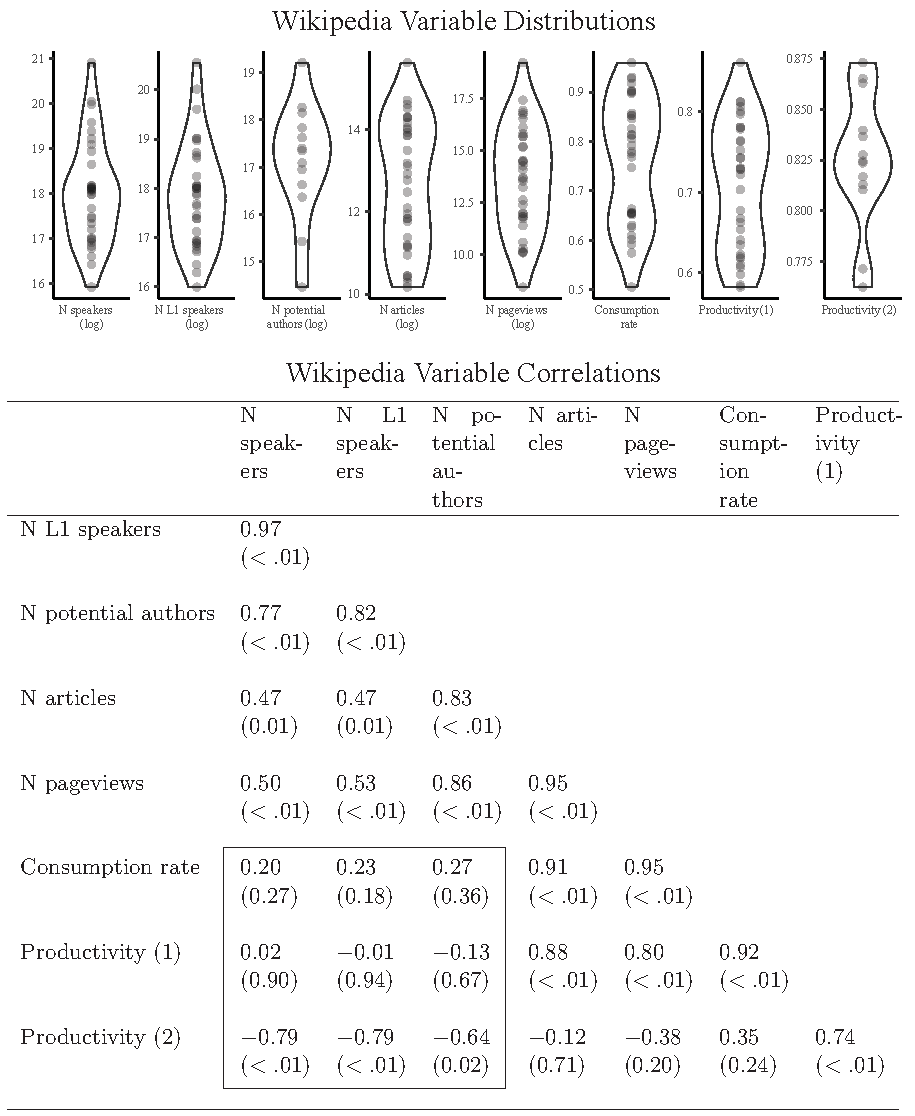
\includegraphics[width = 5.2in]{suppfigs/wiki_distribution_correlation.pdf}


%\pagebreak
%\clearpage
  \caption{{\it Top}: Distributions for eight descriptive statistics associated with multi-lingual Wikipedia corpora. N speakers indicates the log number of first and second language speakers (N languages missing = 1) \cite{wikispeakers}; N L1 speakers indicates the log number of first language speakers only (N missing = 1) \cite{amano2014global}. N potential authors estimates the log number speakers of the target language who have access to the internet, and have sufficient command of the target language to author an article (N  missing = 22) \cite{wikiproductivity}. N articles indicates the log number of articles by language (31 March 2015; N  missing = 1) \cite{wikispeakers}. N pageviews indicates the log number of pageviews by language for a 24 hour period (1 August 2016) \cite{wikipageview}. Consumption rate is the log number of articles / log number of first language speakers (N  missing = 1). Productivity (1) is the log number of articles / log number of first language speakers (N  missing = 2). Productivity (2) is the log number of articles / log number of potential authors (N  missing = 22). Each point corresponds to a language. {\it Bottom}: Pairwise correlations between Wikipedia measures (Pearson's $r$). Parenthetical numbers indicate p-values. Critically, languages with more speakers do not have greater rates of engagement, as measured by number of articles written and viewed relative to the number of speakers. In fact, by one measure of article production (Productivity (2)), languages with more speakers write relatively fewer articles per speaker capita.}
\end{figure}


\pagebreak
 \clearpage


  
   %\section*{Fig. S2}
 \begin{figure}[h]
\centering
     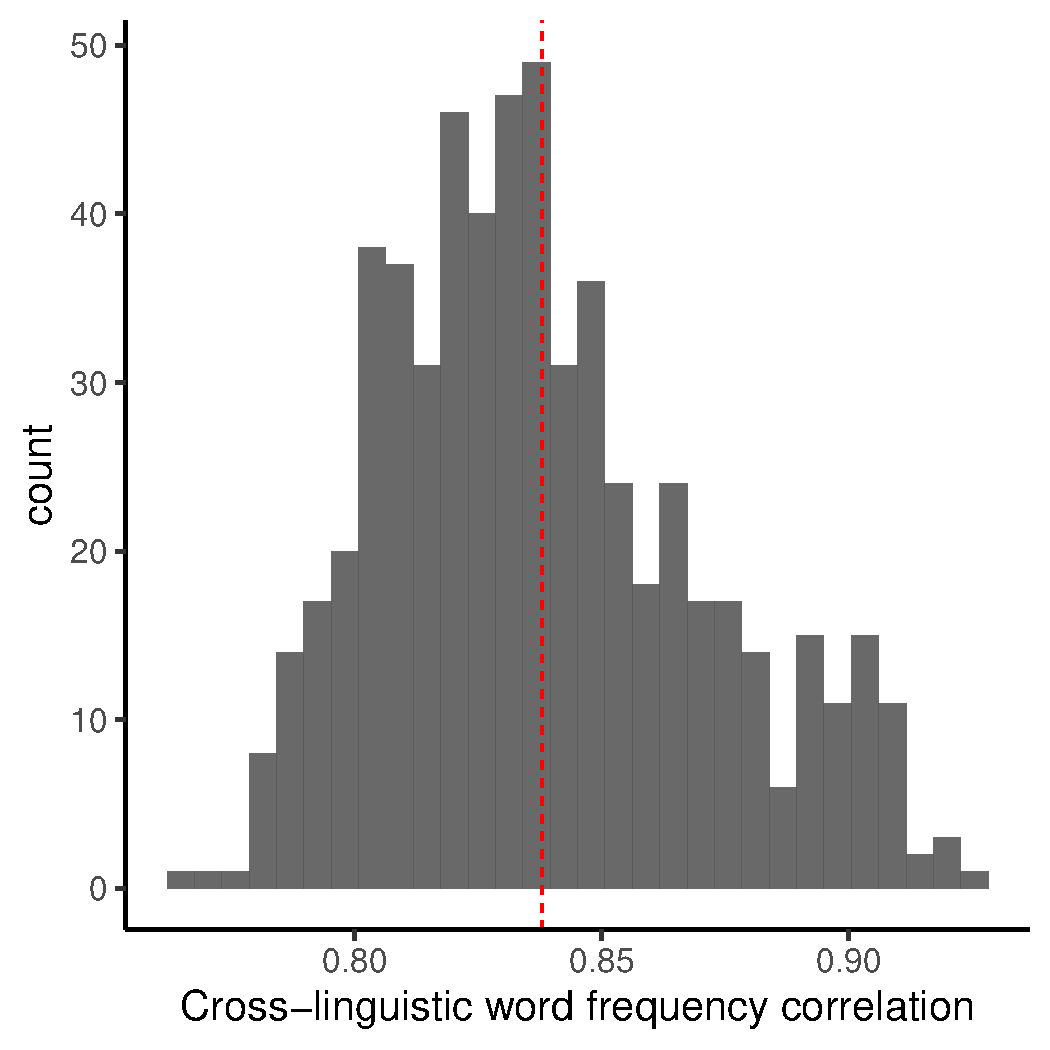
\includegraphics[width = 5in]{suppfigs/ets_xling_freq_plot.pdf}
         \caption{Are findings driven by differences in languages or what speakers of those languages choose to talk about? When we take Spearman’s $\rho$ (rank order correlation) of word frequencies across the ETS essays written by speakers of 35 languages (and limited to words occurring in 10 or more essays across the 38,500 essay sample), we get .84 (for 595 pairs), strongly suggesting that these essays discuss the same topics and broad content, but are hyperlinked with different associations and metaphor as demonstrated by our core findings, illustrated in Fig. 3.

}
\end{figure}


\pagebreak
\clearpage


%\section*{Fig. S3}

\begin{figure}[h]
\centering
\includegraphics[width=16.7cm]{suppfigs/distinctiveness_fig.pdf}


  \caption{Essays written in English by speakers of the same native language are more semantically similar than essays written by speakers of different native languages, corroborating informal observations by second language educators and bilingual researchers in individual pairs of languages second language speakers appear to ``think'' in their first language \cite{wu2014influence, filipovic2018speaking}. We evaluated language semantic distinctiveness by analyzing the position of essays in semantic space for a model trained on all essays in all languages. For each language, we averaged the cosine distance between essay pairs from the same language (``within"), and averaged  pairs between different languages (``between").  We then quantified language-level semantic distinctiveness in two ways: (1) the difference between the two measure (within - between) as in \cite{kozlowski2019geometry, bodell2019interpretable, an2018semaxis, kwak2020frameaxis}, and (2) the ratio between them (within/between) as in \cite{levy2014linguistic, levy2014neural, levy2015improving}. Both types of measures have been shown to capture meaningful semantic relationships in embedding models. In the Main Text, we report the results for the difference measure; here we replicate our results with the ratio measure. The ratio is greater than one when languages are located in a distinct semantic space, relative to other languages. This value was substantially greater than one for all languages in our sample ($M$ = 1.26; $SD$ = .09; $t$(34) = 17.09; $p$ $<$ .00001). We also conducted  this analysis for two types of essays separately: low scoring essays (score $<$ 4 on 5 pt.\ scale) and high scoring essays (score $\geq$ 4).  Low scoring essays ($M$ = 1.27; $SD$ = .08) were more distinct than high scoring essays ($M$ = 1.21; $SD$ = .09; $t$(34) = 5.73; $p$ $<$ .00001).  Main panel shows mean distinctiveness value across samples with the ratio measure.  Red bars correspond to high scoring essays; blue bars correspond to low scoring essays. Ranges indicate bootstrapped 95\% confidence intervals. Upper right panel shows the distribution of essay scores (1-5) for the 38,500 essays in the TOEFL corpus ($M$ = 3.51; $SD$ = .91).}
\end{figure}

\pagebreak
\clearpage


%\section*{Fig. S4}
\begin{figure}[h]
\centering
     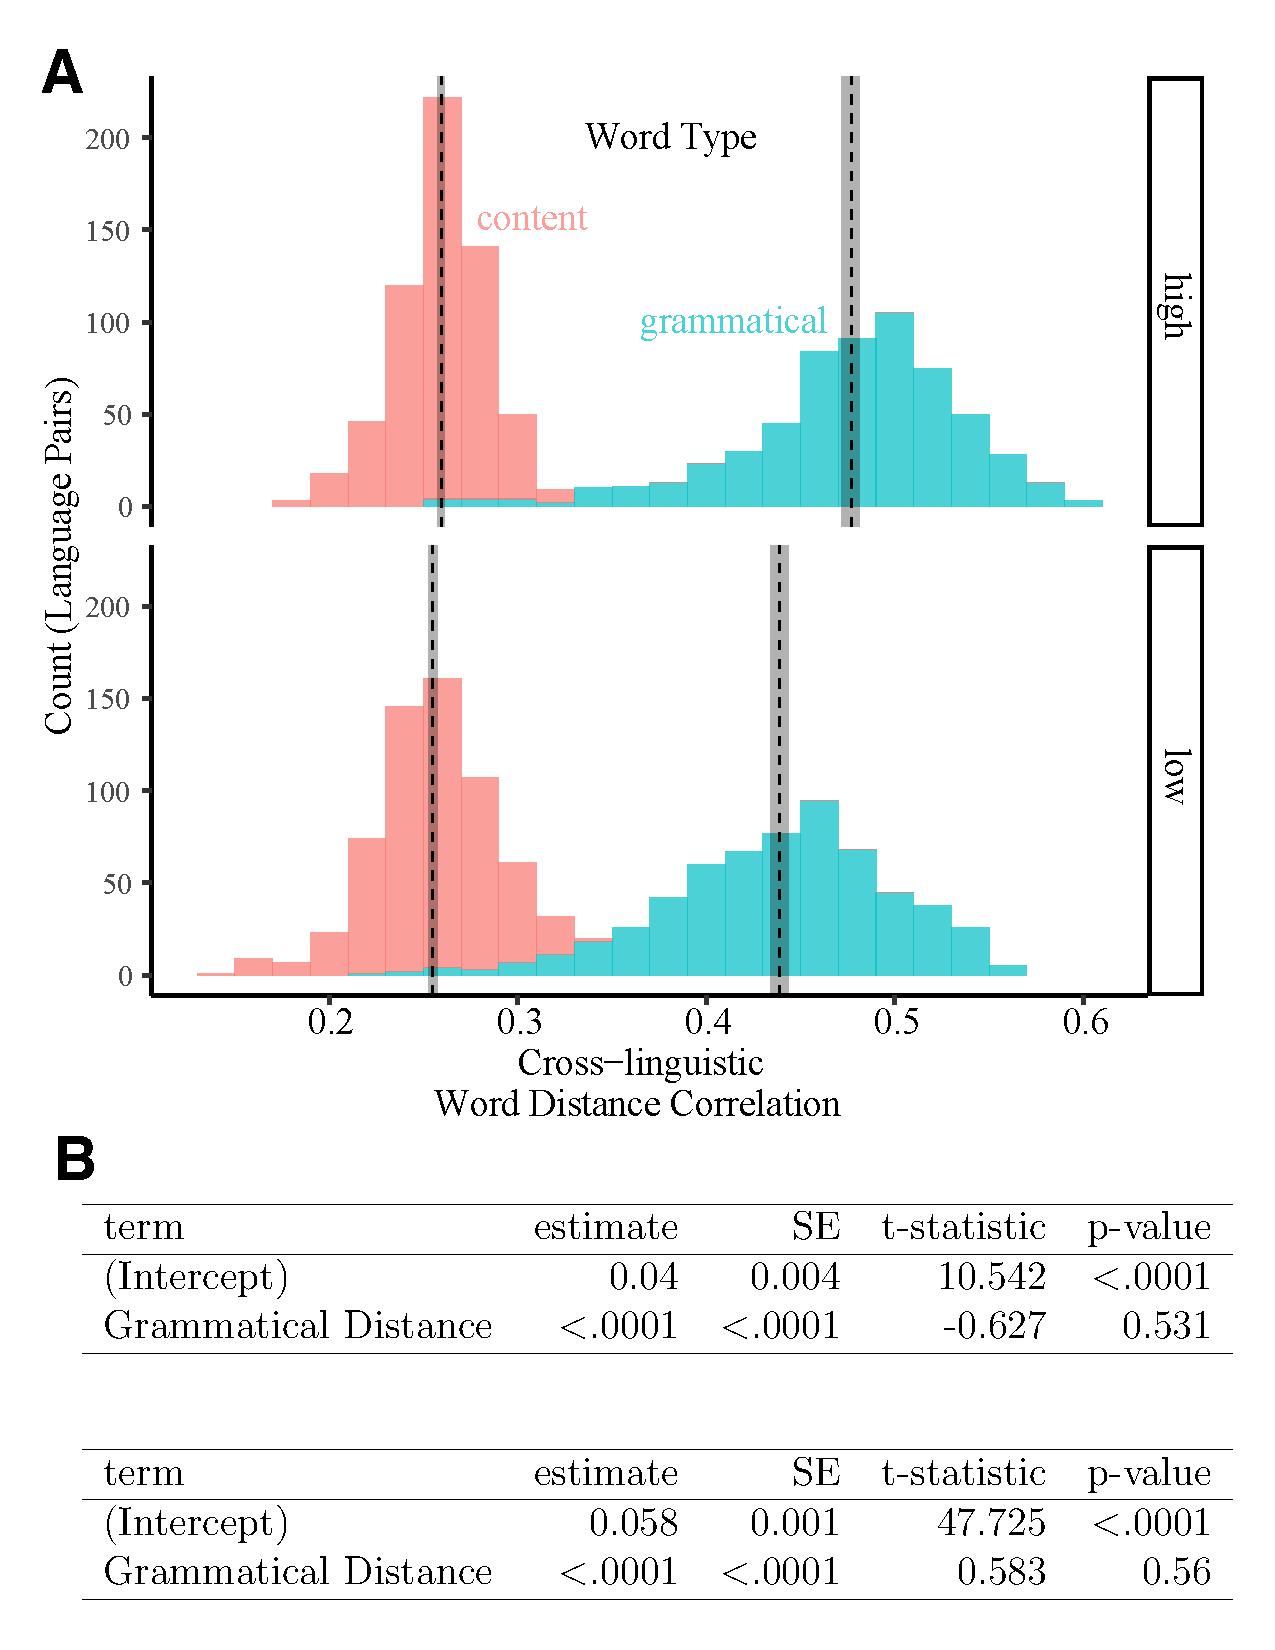
\includegraphics[width=4.5in]{suppfigs/syntax_controlC.pdf}

  \caption{{\textbf A.} Grammatical words (e.g., ``and", ``the") are more similar across languages than content words (e.g., ``love"). In Jakobson's functional typology \cite{jakobson1990language}, grammatical words are \textit{metalingual}--they govern the structure of the code of language itself and so play a related function across languages. As such, grammatical words are qualitatively different from abstract content words such as ``career" or ``government" that vary based on distinctive complex cultural environments. We divided the words from the TOEFL essays analyzed in the Main Text ($N$ = 3,530) into two sets -- ``content" and ``grammatical"  -- based on  part of speech information from \cite{brysbaert2012adding}. Nouns, verbs, adverbs, adjectives, or interjections were categorized as content ($N$ = 3,339); articles, determiners, conjunctions, pronouns, or prepositions ($N$ = 145) were categorized as grammatical. We then calculated the cosine distance between each word pair within a word type (content or grammatical) for models trained separately on low and high scoring essays for essays written by speakers of each of 35 different native languages. Finally, we compared the distances between words across language pairs (e.g., correlation of distances for content words based on essays written by native Spanish versus native French speakers). {\it x}-axis shows magnitude of cross-linguistic word distance correlation (Pearson's $r$); {\it y}-axis shows counts of language pairs. Facets show results from models trained on low (score $<$ 4 on 5 pt.\ scale; bottom) and high (score $\geq$ 4; top) scoring essays. Color indicates word type. Vertical lines indicate distribution means with bootstrapped 95\% confidence intervals. {\textbf B.} Model results predicting the difference between local and global word correlations by language pair ($N$ = 595). Intercept parameter  compares local-global difference to zero; Grammatical distance predictor measures typological distance between languages based on the WALS database \cite{dediu2018trees,wals2013}. Top table shows results for Wikipedia corpus; Bottom table shows results for TOEFL corpus. These models suggest that languages are more similar locally, relative to globally, and that this difference is not predicted by grammatical similarity between languages.}
  \end{figure}

\pagebreak
 \clearpage
 
  %\section*{Fig. S5}

 \begin{figure}[h]
\centering
     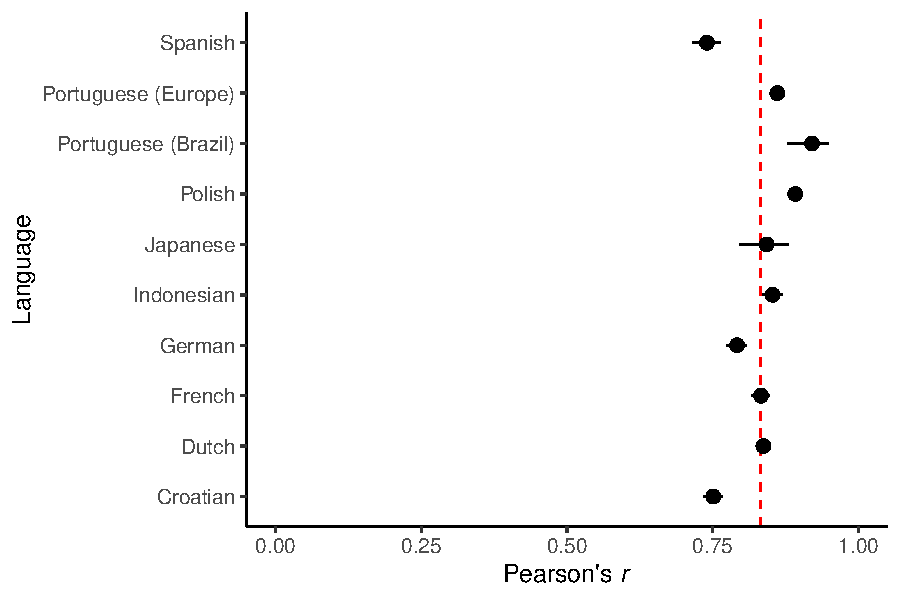
\includegraphics[width = 5in]{suppfigs/conc_corrs.pdf}
         \caption{Comparison of concreteness word norms collected in English versus estimates in other languages. We  aggregated all available concreteness estimates collected by native speakers in a language other than English, and compared the estimate in each language to the estimate of its translation equivalent in English \cite{brysbaert2014concreteness}. Concreteness norms were available for 10 languages: Spanish \cite{guasch2016spanish}, Portuguese (European) \cite{soares2017minho}, Portuguese (Brazil) \cite{lima2021norms}, Polish, \cite{imbir2016affective} Japanese \cite{allen2014cross}, Indonesian \cite{sianipar2016affective}, German \cite{charbonnier2020predicting}, French \cite{bonin2018concreteness}, Dutch \cite{brysbaert2014norms}, and Croatian \cite{coso2019affective}. The figure shows the correlation (Pearson's $r$) between word estimates in each language, compared to English. Ranges correspond to 95\% confidence intervals, and the red dashed line indicates the  mean correlation across languages. Overall, estimates of concreteness collected in English were highly correlated with estimates collected in other languages ($M$ = .83), suggesting a word's conceptual concreteness is largely language independent. }
\end{figure}

\pagebreak
\clearpage


%\section*{Fig. S6}
\begin{figure}[h]
\centering
\includegraphics[width=5in]{suppfigs/concreteness_plot_random.pdf}

 \caption{An alternative explanation for the finding that concrete words are more similar cross-linguistically  relative to abstract words is that concrete words, in general, tend to appear in more similar contexts in corpora of text relative to abstract words. To test this possibility, we constructed 35 corpora with each corpus containing equally-sized samples of TOEFL essays  from each of the 35 different languages. Each corpus was therefore comparably sized to the language-based corpora described in the Main Text (approx.\ 1100 essays), but contained essays written by speakers of all 35 native languages. We then calculated mean pairwise correlation between word distances across languages as a function of the concreteness decile of the words. Point ranges correspond to bootstrapped 95\% confidence intervals; range on model fit corresponds to the standard error. Unlike for the language-based corpus, there is no effect of concreteness on cross-corpus similarity: Across corpora, low and high concrete meanings are equally similar ($r$ = .02; $p$ = .96). This suggests that the concreteness effect reported in the Main Text is due to cross-linguistic differences in meanings, rather than an artifact of, e.g., differing types of linguistic contexts for high versus low concrete words. }

\end{figure}


\pagebreak
\clearpage


%\section*{Fig. S7}

\begin{figure}[h]
\centering
\includegraphics[width=5in]{suppfigs/conc_freq_control.pdf}
 \caption{Mean word frequency for words in each concreteness decile from the TOEFL corpus. Word frequency is estimated from the actual word counts in the corpus. Error bars are bootstrapped 95\% confidence intervals. This analysis suggests that more concrete words tend to be less frequent in the corpus, making it unlikely that the relationship between concreteness and cross-linguistic similarity is due to measurement noise.}
\end{figure}

\pagebreak
 \clearpage

  %\section*{Fig. S8}
 \begin{figure}[h]
\centering
     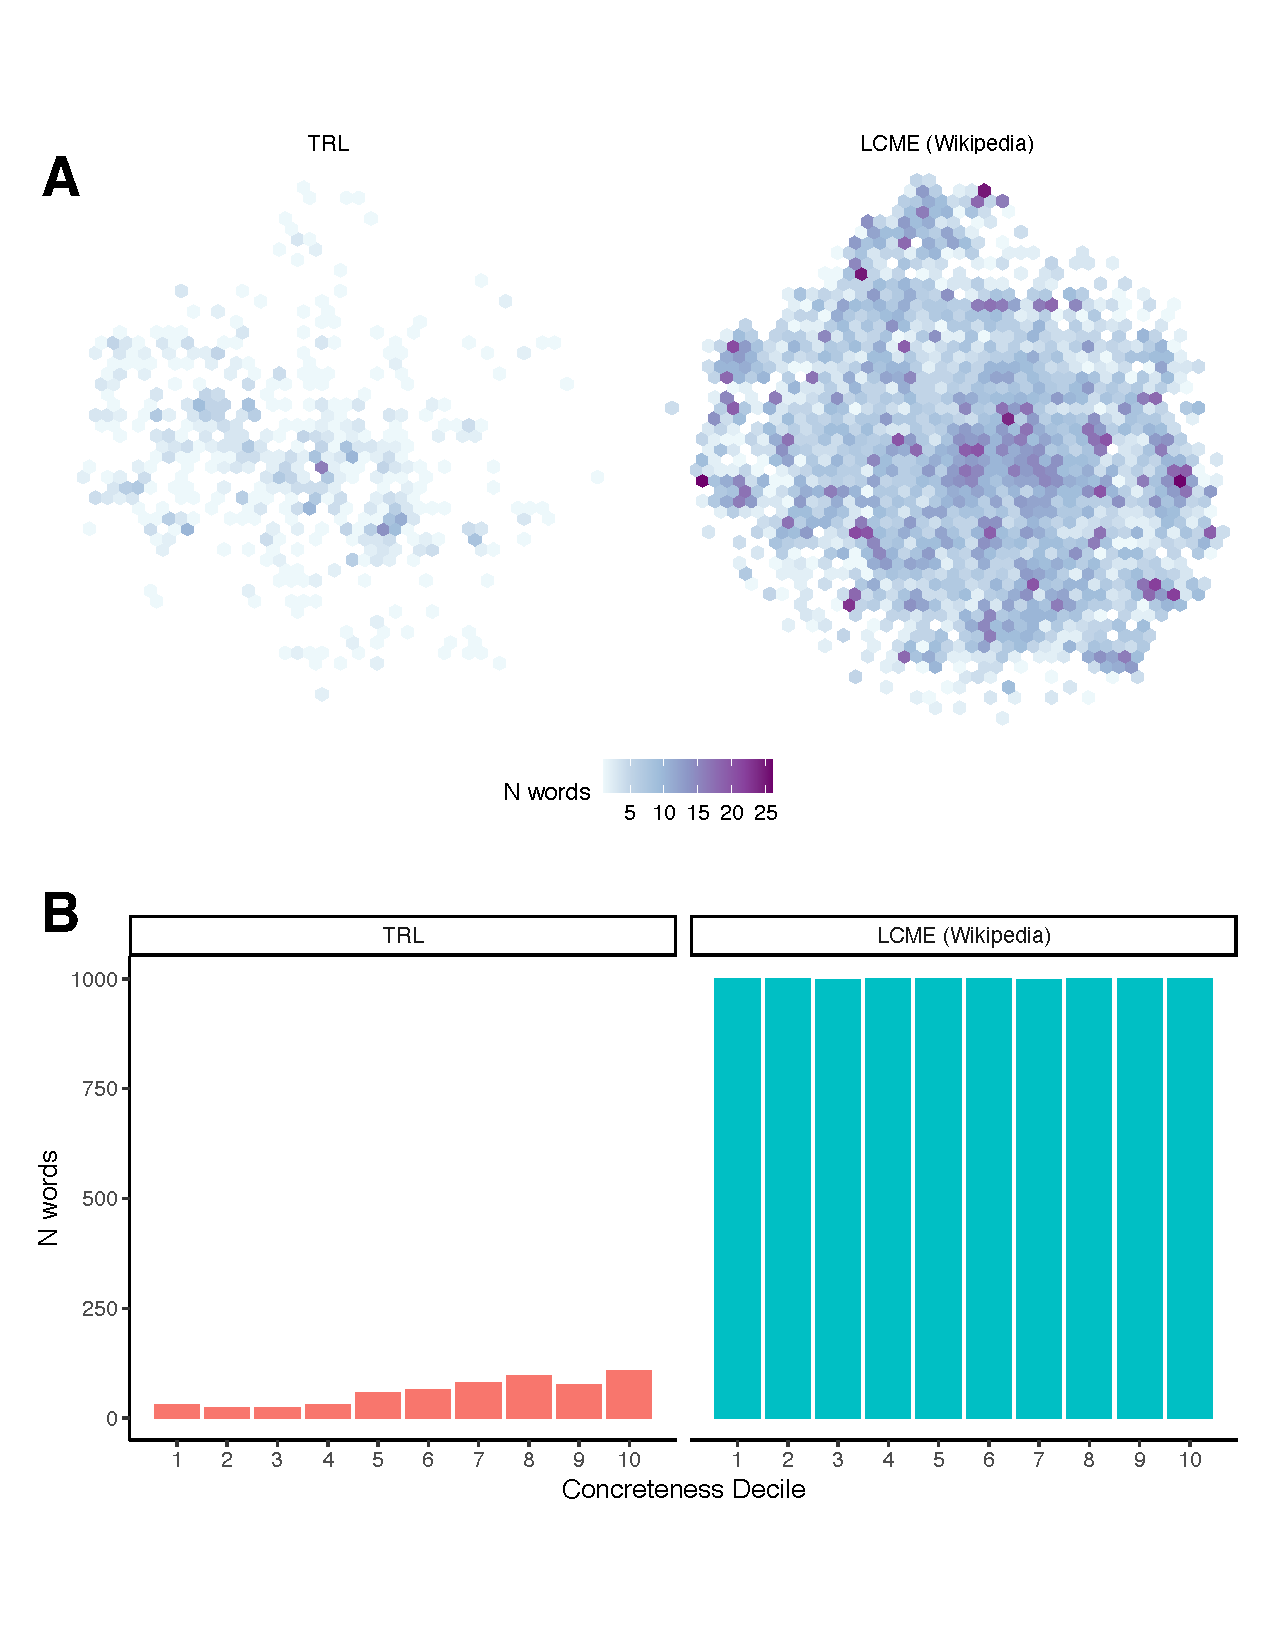
\includegraphics[width = 6in]{suppfigs/thompson_word_comparisonC.pdf}
         \caption{Comparison of our samples (LCME) with those in \cite{thompson2020cultural}, or TRL hereafter. \textbf{A}. Density plot covering our word samples from the English corpus, projected to two dimensions using TSNE; \textbf{B}. Histograms of the samples over the deciles of the concreteness distribution. TRL sampled concepts/words by 21 hand-selected domains (e.g., animals, food \& drink, possessions, kinship, quantities, time) with the expressed purpose of exploring the relationship between the local coherence and category type across their sample of 10 language families (41 languages). They did this by selecting the 100 closest neighbors to each target word, and correlating these ranked lists across languages, then averaging them across target words within domain (e.g., “mother”, “father”, “aunt”, “uncle” for the kinship domain). This local measurement revealed that the abstract domains of quantity, time and kinship correlated most highly across languages because of their internal coherence. They then inferred that abstract concepts in general were more coherent than concrete concepts. Plots A and B show that TRL's words unwittingly clumped in semantic space and within the higher deciles of the concreteness distribution -- they were not selected to test the concreteness hypothesis. By contrast, we use 10,000 concepts randomly sampled from each decile of the concreteness norm distribution for the purpose of testing the relationship between concreteness/abstractness and variance in meaning across languages. Our samples show that the concrete-abstract association does correlate with word variation across languages, but explains less than word position. Words within domains (independent of concreteness) cluster together across languages much more tightly than between them, creating local coherence but global variance across the world's language.}
\end{figure}

\pagebreak
\clearpage


%\section*{Fig. S9}

\begin{figure}[h]
\centering
     \includegraphics[width=6in]{suppfigs/swadesh_plot_ED.pdf}
 \caption{Physical distance between where  two languages are spoken predicts semantic similarity of Swadesh \cite{swadesh1952lexico} meanings between two languages: Languages that are geographically closer have more similar meanings. Each facet corresponds to a Swadesh word. Each point shows the correlation between the pairwise distances between the target Swadesh word and all other Swadesh words for a language pair (e.g., a point on the ``earth" facet represents the magnitude of the correlation between Spanish and French of  the distances between ``earth" and all other Swadesh words). Physical distance  in meters (millions) between languages is plotted on the x-axis and magnitude of correlation between distances to other Swadesh items is plotted on the y-axis. All correlations are significant at the $\alpha$ = .01 level except the items ``star" (QAP $p$ = .016) and ``lake" (QAP $p$ = .119).}
 \end{figure}


\pagebreak
\clearpage




%\section*{Fig. S10}

\begin{figure}[h]
\centering
     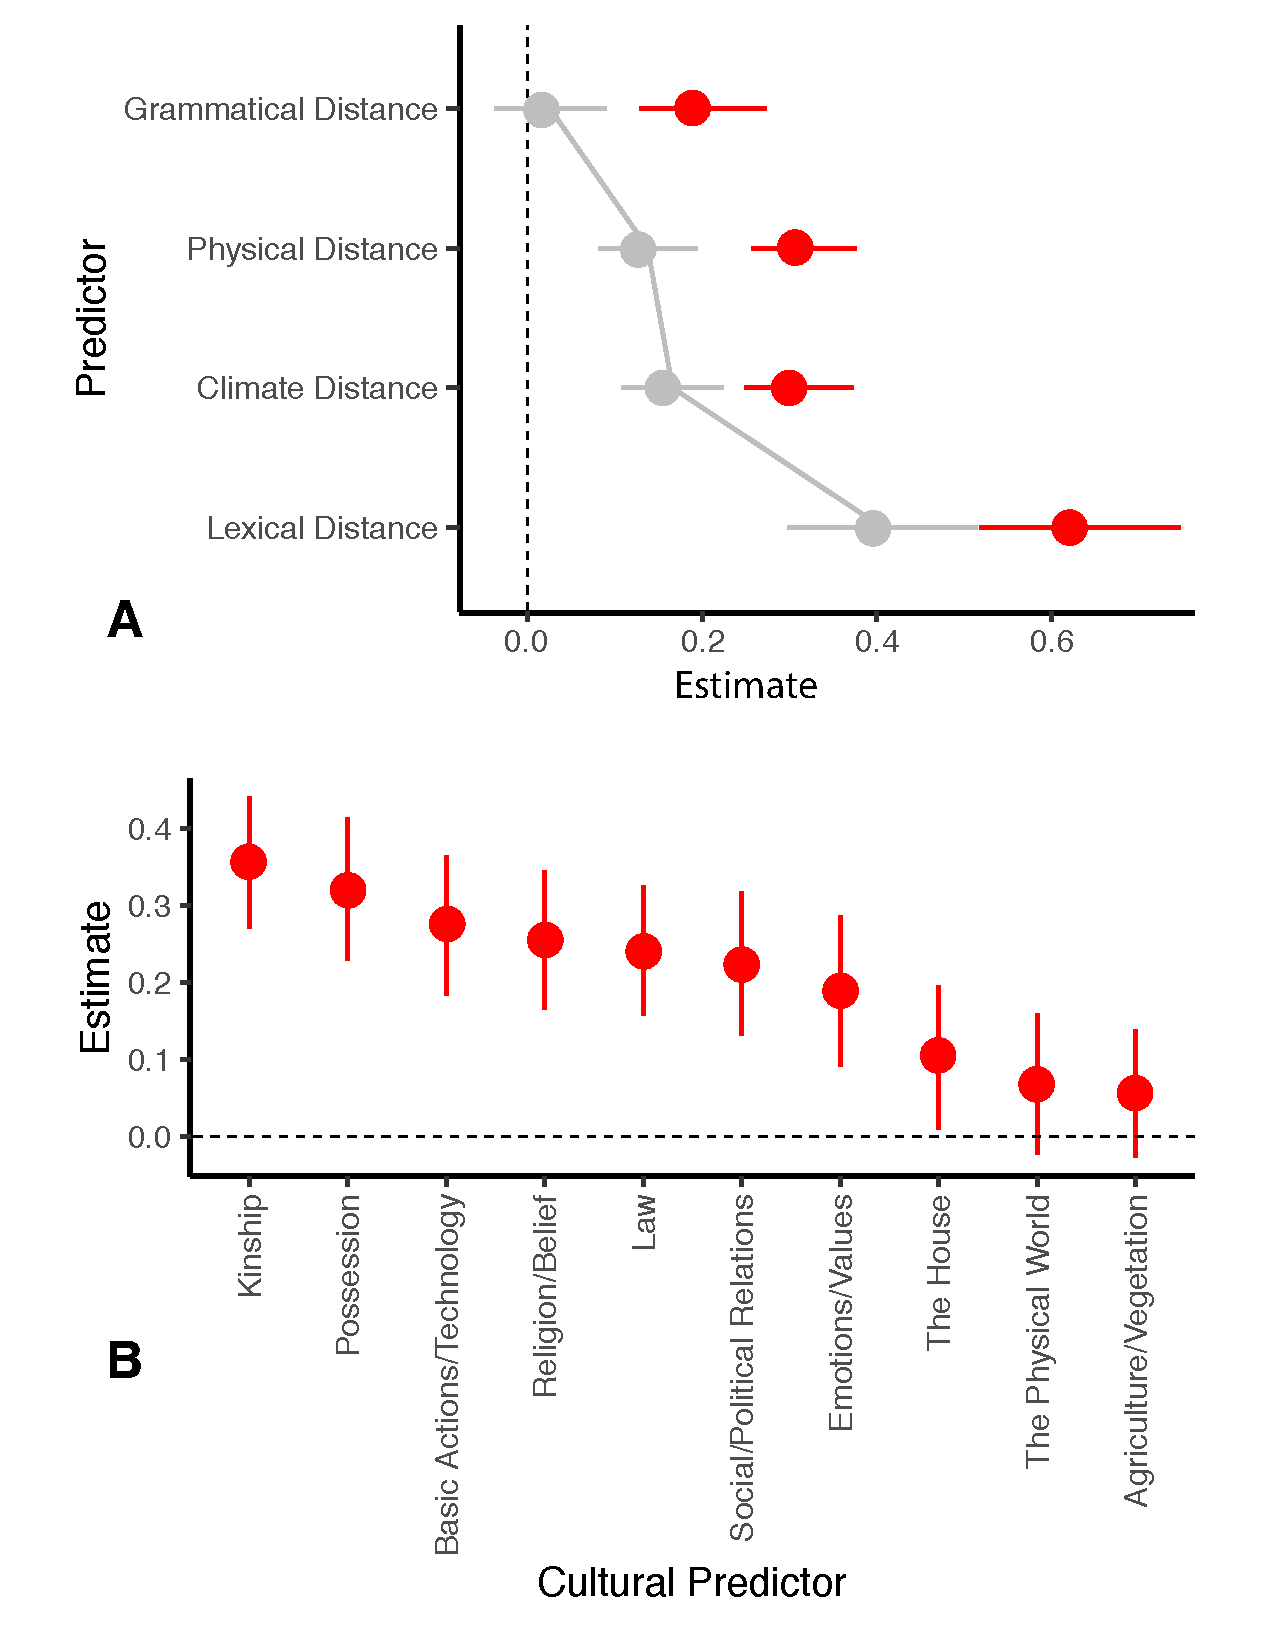
\includegraphics[width=4.5in]{suppfigs/distance_regressionsC.pdf}


 \caption{{\textbf A.} Language pairwise predictors of semantic similarity for full sample of 35 languages. Cultural language distances were not available for 7 of the 35 languages in our sample (German, Greek, Italian, Portuguese, Romanian, Farsi, and Yoruba). In the Main Text, we report model parameters for the set of 28 languages for which we have full data. Here, we show model parameters for the other predictors for the full sample of 35 languages.  Red points indicate standardized estimates from a single-predictor model; grey points indicate estimates from additive linear model with all five predictors included. Ranges are 95\% confidence intervals. {\textbf B.} Cultural predictors of semantic distance for each of 10 cultural sub-domains.  Points are standardized estimates from an additive linear model with all five predictors included. Ranges are 95\% confidence intervals.}
 
 \end{figure}



\pagebreak
 \clearpage
  
%\section*{Fig. S11}
 \begin{figure}[h]
\centering
     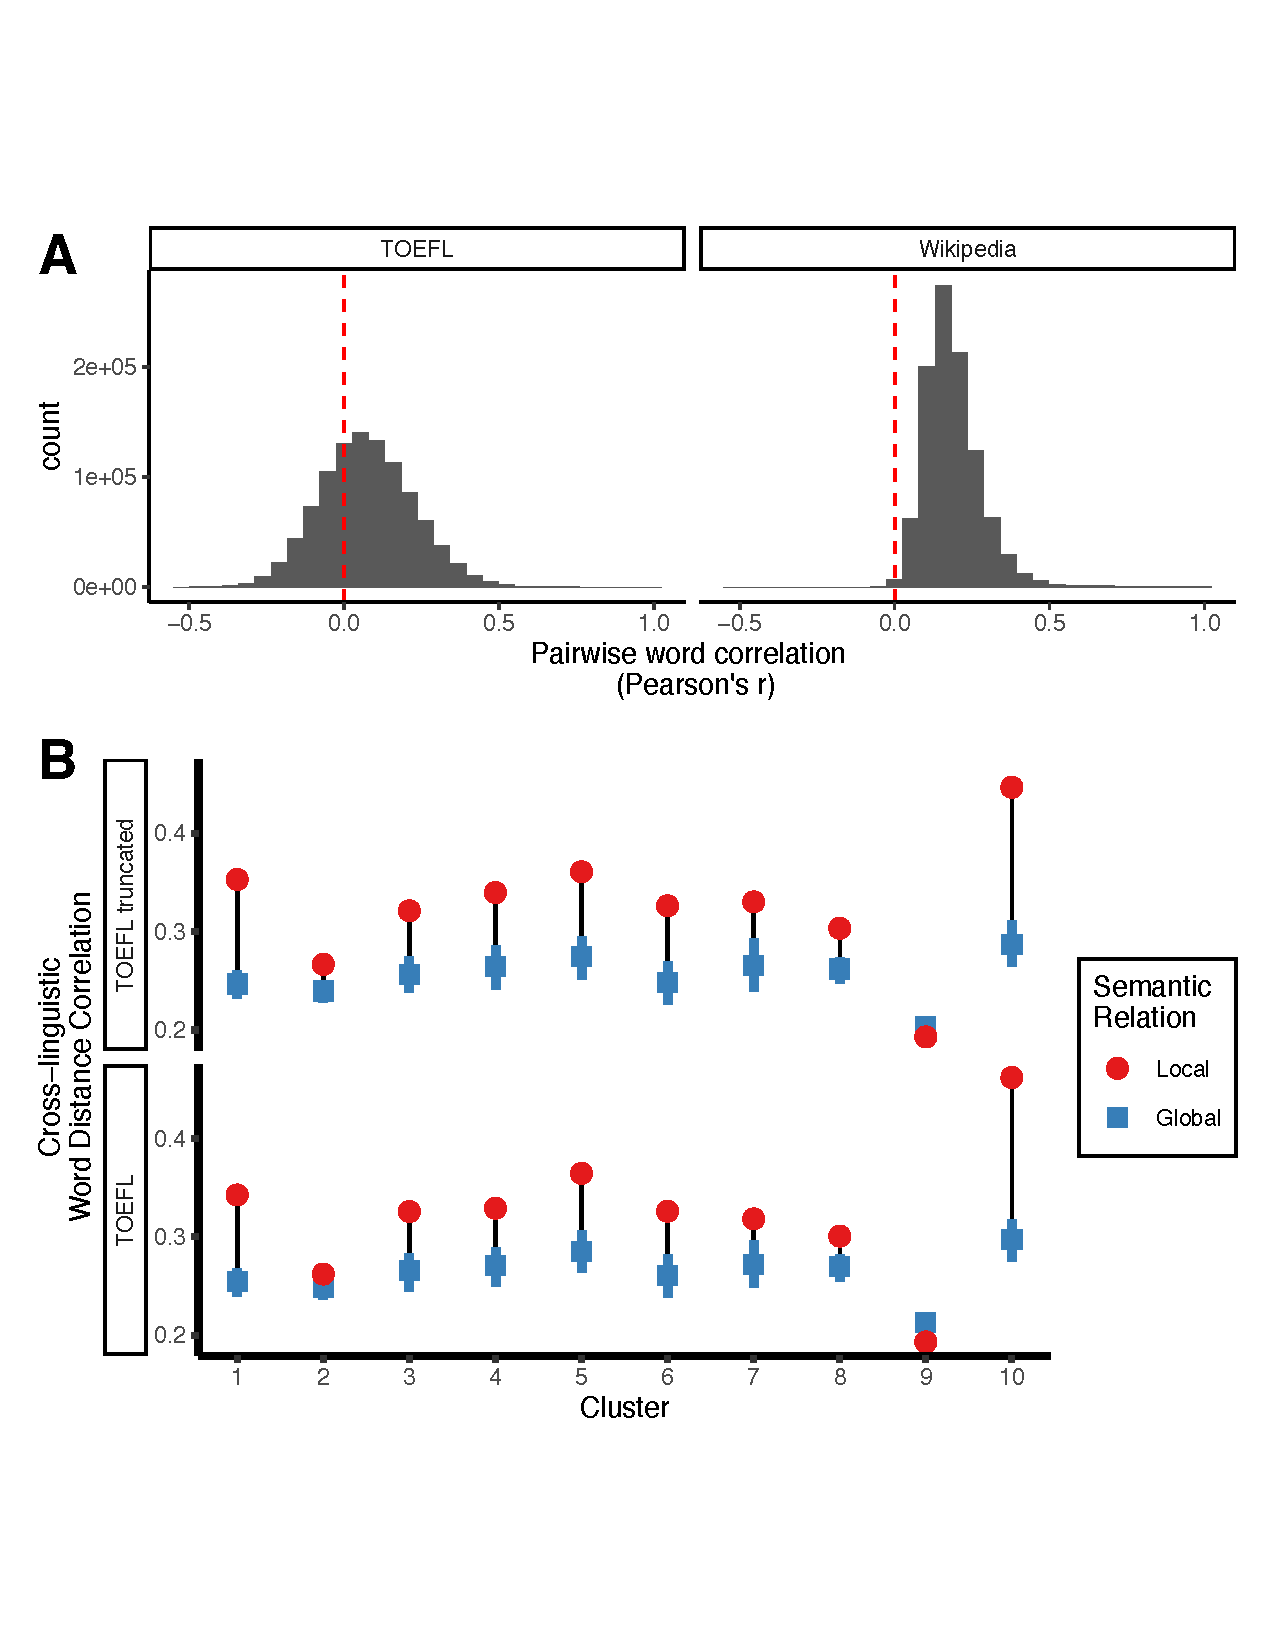
\includegraphics[width = 6.5in]{suppfigs/local_global_plot_truncatedC.pdf}
         \caption{Local vs. global distances, examining (A) then truncating (B) negative distances. \textbf{A}, the distribution of pairwise distances within language models from a random sample of 1M word pairs in the TOEFL models (left) and Wikipedia models (right). For Wikipedia, 99.8\% of pairwise distances were greater than zero. However, in the case of the TOEFL models, only 67.9\% were greater than zero, meaning there were a large subset of large distances included in our analyses (32.1\%). \textbf{B}, Because very large distances (e.g., those larger than $90^{\circ}$ with a cosine $\theta < 0$) are unlikely to be meaningfully different than those defined as unrelated and equal to $90^{\circ}$ and $\theta = 0$ because they were not trained with inverse associations, we re-ran our core analysis (see Fig. 3C), rounding cosine distances greater than $90^{\circ}$ (i.e., negative values) to $90^{\circ}$ -- the theoretical bound for unrelatedness. The result represents a nearly 20\% increase in the local-global effect (Truncated TOEFL: M = 0.069, SD = 0.008; t(594) = 205.24; p < .0001; d = 3.4 [3.22, 3.58]; W = 177310, p < .0001; TOEFL: M = 0.058, SD = 0.008; t(594) = 185.97; p < .0001; d = 2.84 [2.68, 3]; W = 177310, p < .0001). This suggests that the analyses reported in the main text, which included these very large distances, lead to a conservative estimate of the local-global effect for the TOEFL data.

}
\end{figure}


\pagebreak
 \clearpage

%\section*{Fig. S12}
\begin{figure}[h]
\centering
     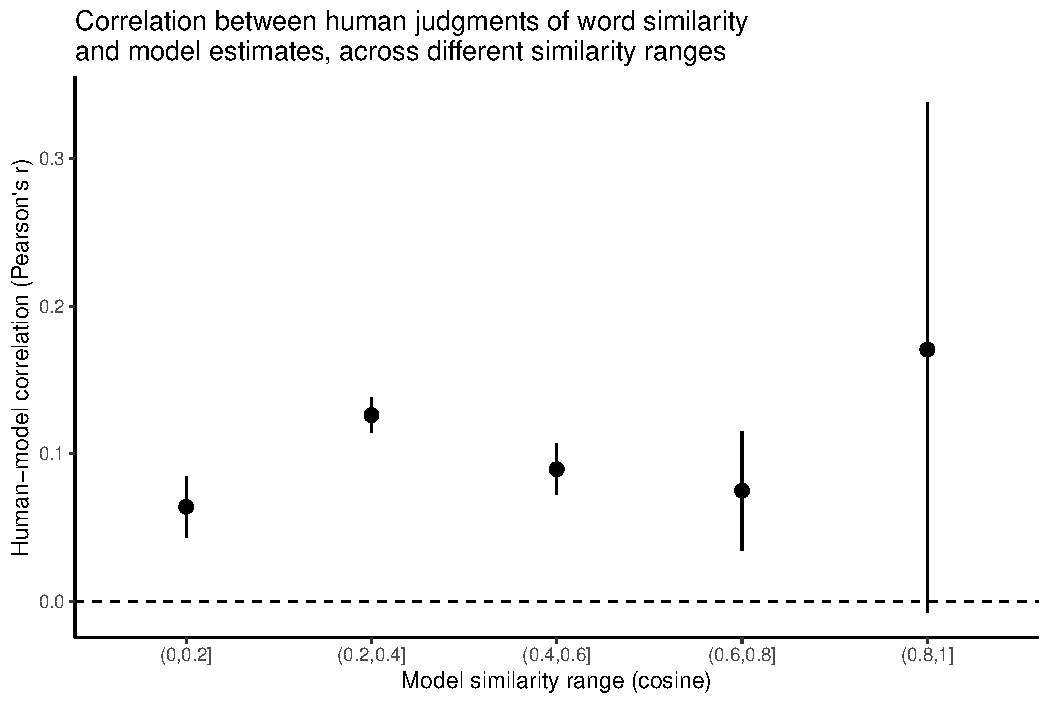
\includegraphics{suppfigs/distance_validation_plot.pdf}
         \caption{Stable correlations between close and distant words in our sample.
         Data from word-pairs crowd-sourced by participants in the Small World of Words project -- https://smallworldofwords.org/en/project/ \cite{de2019small} -- in which participants were given a target word (e.g., ``cat'') and asked to list three associated words (e.g., ``kitten'', ``milk'', ``mouse''). We analyzed the first associates for each target word, which are likely to be most closely associated with the target. By aggregating across many participants, we can estimate the similarity between the target and associate as the conditional probability of the associated word, given the target (P(``kitten''|``cat''). We then get an estimate of model similarity by projecting target and associated words onto a FastText model built from English Wikipedia \cite{bojanowski2016enriching}, and calculating their cosine distance. The plot shows the correlations between human and model estimates for word pairs at varying cosine distances. As a group, words farther from the focal word (i.e., more distal words) are comparably correlated to human judgments than words much closer. To the extent that these models capture psychological similarity between word meanings, this means that they do so equally well for words close and farther in meaning from the target word. 
}
\end{figure}

\pagebreak
 \clearpage

%\section*{Fig. S13}
 \begin{figure}[h]
\centering
     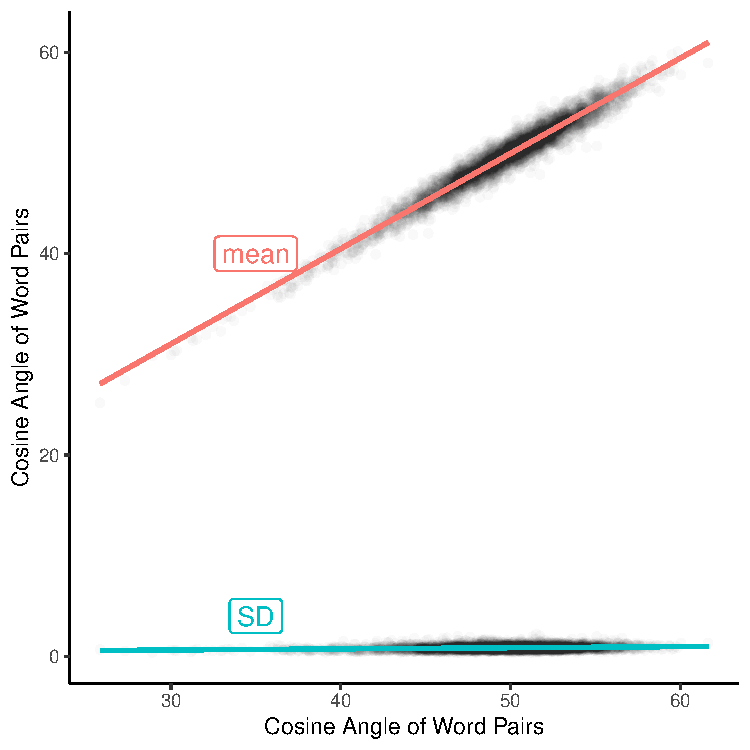
\includegraphics{suppfigs/austin_mean_sd_distancs.pdf}
         \caption{Analysis of the relationship between mean and standard deviation for the cosine angle between pairs of word vectors from word embeddings built from a corpus of Google Books n-grams (2000-2010). Means and standard deviations  for 100 words randomly sampled from our ETS analysis, computed from 20 word2vec models built from nonoverlapping subsets of the corpus \cite{politis1999subsampling} -- details in \cite{kozlowski2019geometry} -- resulting in 4,900 unique word pairs between distinct words. Greater mean cosine distances (measured in degrees) between words enables a much greater theoretical variance and standard deviation between those distances across models. Nevertheless, our subsampled standard deviations barely increase at all. This strongly suggests that distant associations are at least as stable and precise across models (and the distinct subsamples of text on which they are trained) as proximate associations. Distant associations cannot be attributable to random seeds or fluctuations of the algorithm.
}
\end{figure}

\pagebreak
 \clearpage

%\section*{Fig. S14}
\begin{figure}[h]
\centering
     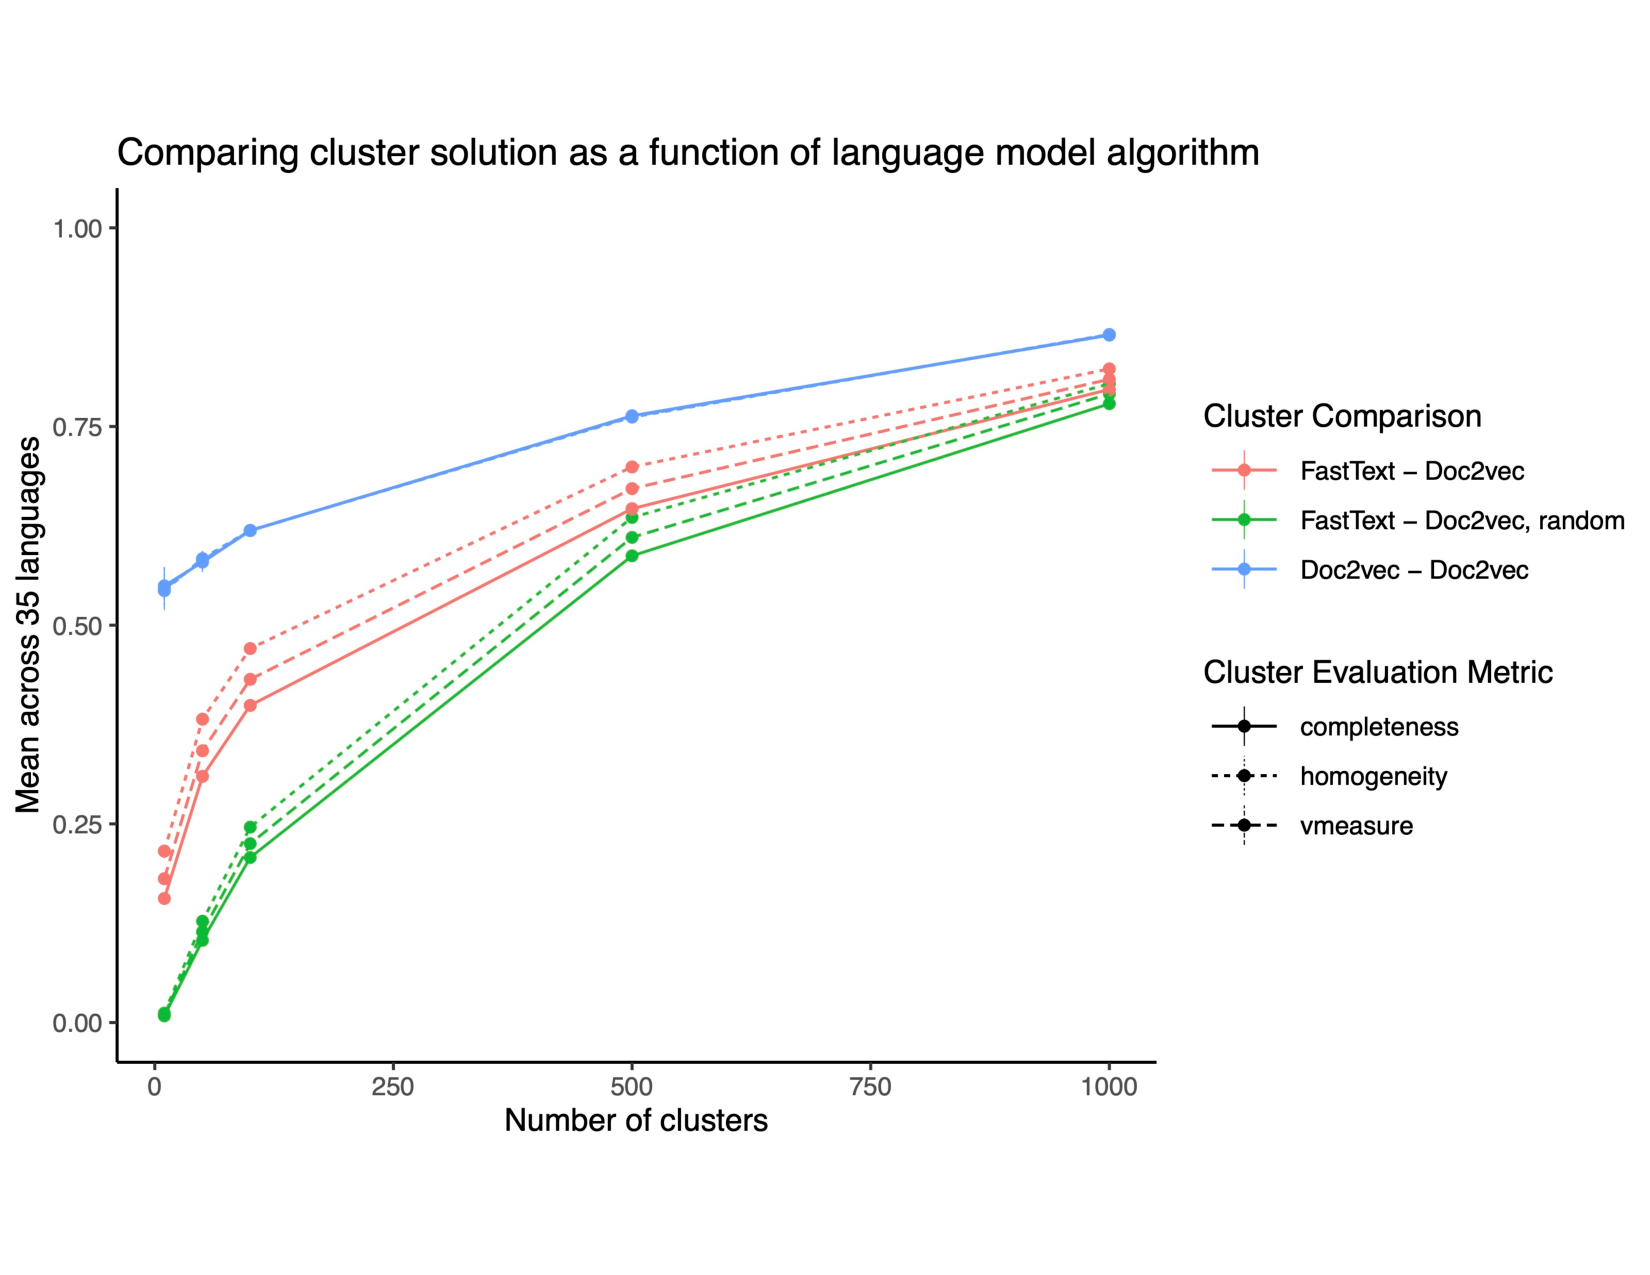
\includegraphics[width = 7in]{suppfigs/cluster_alogrithm_comparison.pdf}
         \caption{Comparison of FastText and Doc2Vec algorithms. We directly compare FastText and Doc2Vec algorithms by training new models with each on the ETS essay data. For both models, the distance between the same word pairs correlate substantially and significantly. We analyzed the similarity of clusters constructed from FastText model outputs with those constructed from Doc2Vec model output using the V-measure \cite{rosenberg2007v}, which 1) does not depend on the clustering algorithm or data set, 2) evaluates the clustering of all data points, and 3) constructs an accurate evaluation and combination (the geometric mean) of homogeneity and completeness. For example, a FastText clustering result satisfies homogeneity if all of its clusters contain only data points that are members of a single Doc2Vec cluster. A clustering result satisfies completeness if all the data points that are members of a given FastText cluster are elements of the same Doc2Vec cluster. In this way, the homogeneity and completeness of a clustering solution run approximately in opposition: Increasing homogeneity often results to decrease its completeness. We compare 10, 50, 100, 500, and 1000 cluster solutions from FastText and Doc2Vec with respect to each other and upper and lower baselines: (1) Doc2Vec vs. Doc2Vec clusters, constructed with different random seeds, which represents an upper bound, and (2) Doc2Vec vs. random clusters, which represents a lower bound. For the 10 cluster solutions, mean V-measures are approximately .2, rising to nearly .4 in the 100 cluster solution. For all but the largest cluster solutions (1000), these are much higher than the random baseline. Note that as we increase the cluster solution from 10 to 100 clusters, we increase the similarity between the FastText and Doc2Vec clusterings relative to the upper baseline and decrease its similarity to the lower one.
}
\end{figure}


\pagebreak

\clearpage

%\section*{Fig. S15}

\begin{figure}[h]
\centering
\includegraphics[width = 6.3in]{suppfigs/continuous_semantic_clusters.pdf}
   \caption{As described in the Main Text, we clustered words into 10 clusters for each of the two corpora (Second-Language TOEFL and Multilingual Wikipedia). Each point in the figure corresponds to a unique pair of clusters. The y-axis shows the average correlation (Pearson's {\it r}) in pairwise word distances between the two clusters across all language pairs (e.g., correlation of all word pair distances between the 1-2 cluster pair for French and Spanish, and all other language pairs). The x-axis shows the cosine distance between the centroids of the two clusters. Color indicates whether the two clusters are the same  (``local;" red) or different (``global;" blue). There is a positive correlation between cluster centroid distance and the magnitude of the pairwise word correlation for both corpora (TOEFL: $r$ = .39, $p$ = .003; Wikipedia: $r$ = .34, $p$ = .01). Notably, however, there is a bimodal relationship in centroid distances characterized by the local-global distinction.}
\end{figure}


\pagebreak
\clearpage


% latex table generated in R 3.6.1 by xtable 1.8-4 package
% Mon May 25 13:36:50 2020
%\begin{sidewaystable}



%\section*{Fig. S16}

\begin{figure}[h]
\centering
     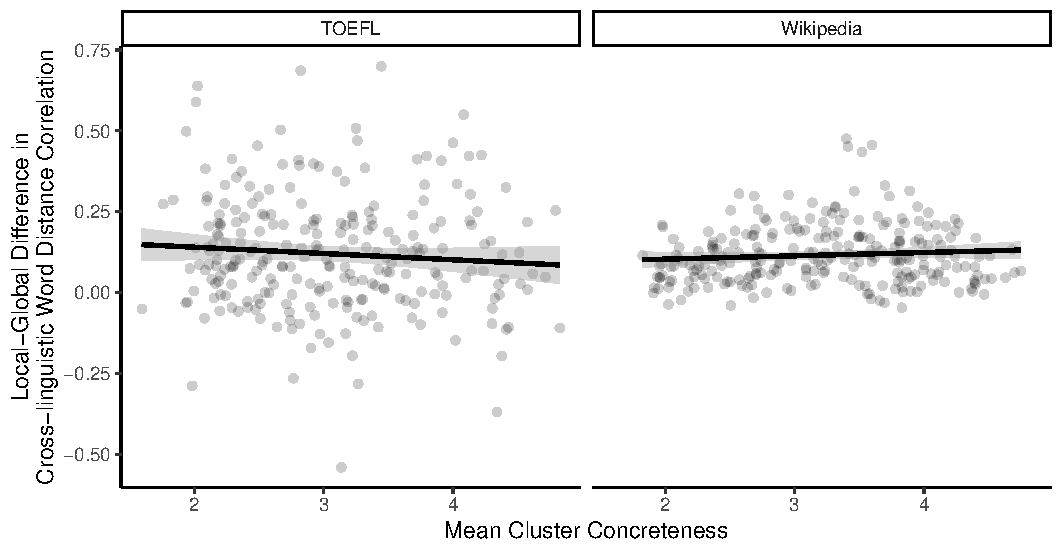
\includegraphics[width = 6.3in]{suppfigs/local_global_concreteness_semantics_plot.pdf}
         \caption{Relationship between cluster concreteness and the magnitude of the local-global effect for the 250 cluster solution for TOEFL (left) and Wikipedia (right). For each cluster in each corpus, we calculated the mean concreteness of words in that cluster and the mean cross-linguistic correlation in word pairwise distances within the same cluster (local) versus across different clusters (global). The {\it y}-axis shows the difference in local versus global correlations  aggregating across language pairs. Larger values indicate that word meanings are more similar within clusters versus across them. Each point corresponds to a cluster. These results reveal that, while semantic clusters tend to co-vary with concreteness, the concreteness of a cluster is not predictive of the local-global effect. }
\end{figure}


\pagebreak
 \clearpage

%\section*{Fig. S17}
  \begin{figure}[h]
\centering
     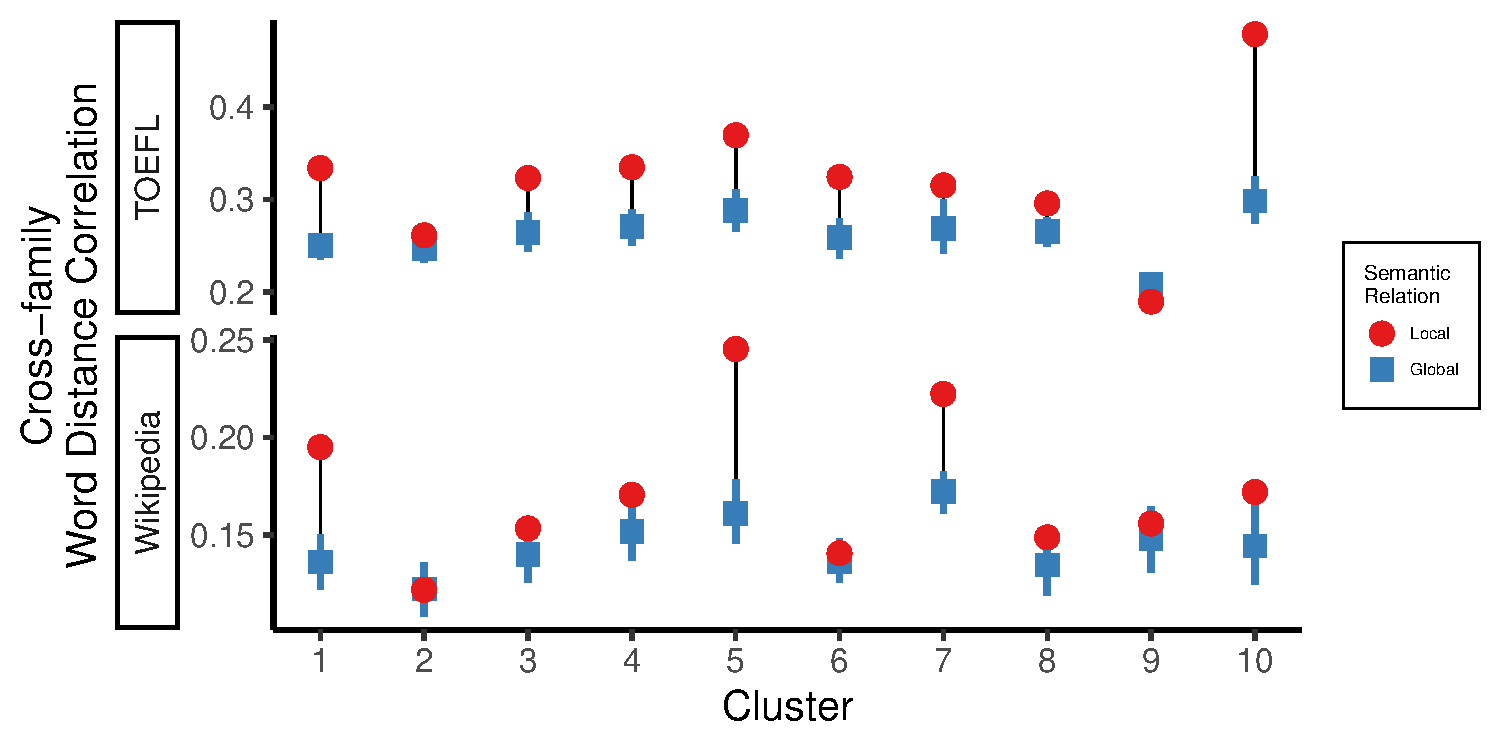
\includegraphics[width = 7in]{ suppfigs/local_global_family.pdf}
         \caption{Cross-family (11 language families) word distance correlations for word groups in 10 semantic clusters based on word embeddings obtained from Second-Language TOEFL Corpus (top) and Multilingual Wikipedia Corpus (bottom). Red points indicate mean local correlation for each cluster, and blue squares indicate global correlation for each cluster (TOEFL:  $M$ $=$ 0.061, $SD$ $=$  0.007;  $t$(54)  $=$ 64.37; $p$ $<$ .0001; $d$  $=$ 2.98 [2.44, 3.52]; Wikipedia: $M$  $=$  0.03, $SD$   $=$  0.033;  $t$(54)  $=$ 6.91; $p$ < .0001; $d$ = 0.29 [-0.09, 0.66]).Note that the cluster number labels are arbitrarily assigned, and that the words assigned to each cluster differ across the two corpora. Despite far fewer observations than in the main analysis, we see the same, statistically significant pattern in both corpora: local distance are more highly correlated across language families, relative to global distances. Even though several linguistic families manifest a single language representative (e.g., Afro-Asiatic, Altaic, Austro-Asiatic, Japonic, Sino-Tibetan, Tai-Kadai, Korean), with necessarily smaller Wikipedia text corpora, the pattern is manifest even with these more limited textual samples.   

}
\end{figure}

\pagebreak
 \clearpage
 
   %\section*{Fig. S18}
 \begin{figure}[h]
\centering
     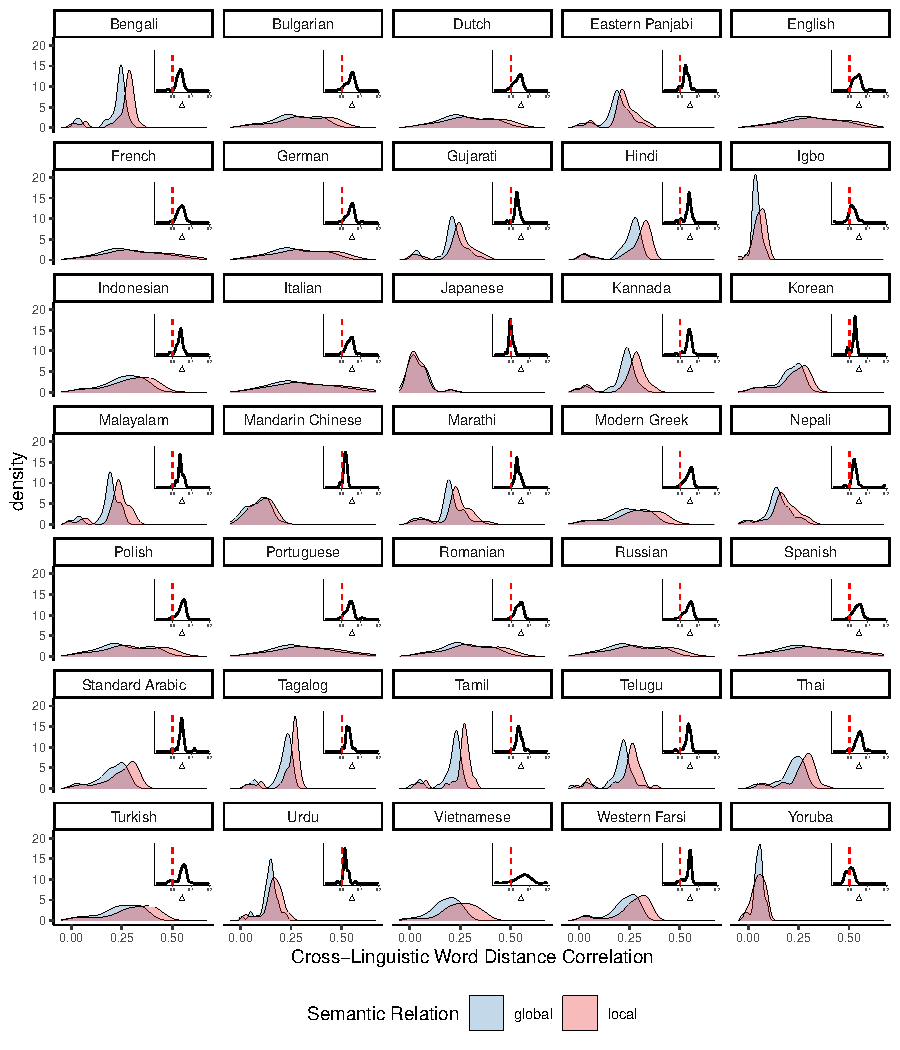
\includegraphics[width = 7in]{suppfigs/local_global_language_dist_ED_WIKI.pdf}
         \caption{Distribution of local-global correlation difference by language, for the Wikipedia corpus. Each subplot shows the difference in correlation between local distances and global distances for one language with all other languages ($n$ = 34). The insets manifest the differences in the two distributions with the dashed red line signifying a difference of 0. These demonstrate that Wikipedia local-global differences are not driven by outliers but appear largely balanced across all language combinations, with a consistent effect of roughly the same size across language comparisons.
}
\end{figure}

\pagebreak
 \clearpage
 
   %\section*{Fig. S19}
 \begin{figure}[h]
\centering
     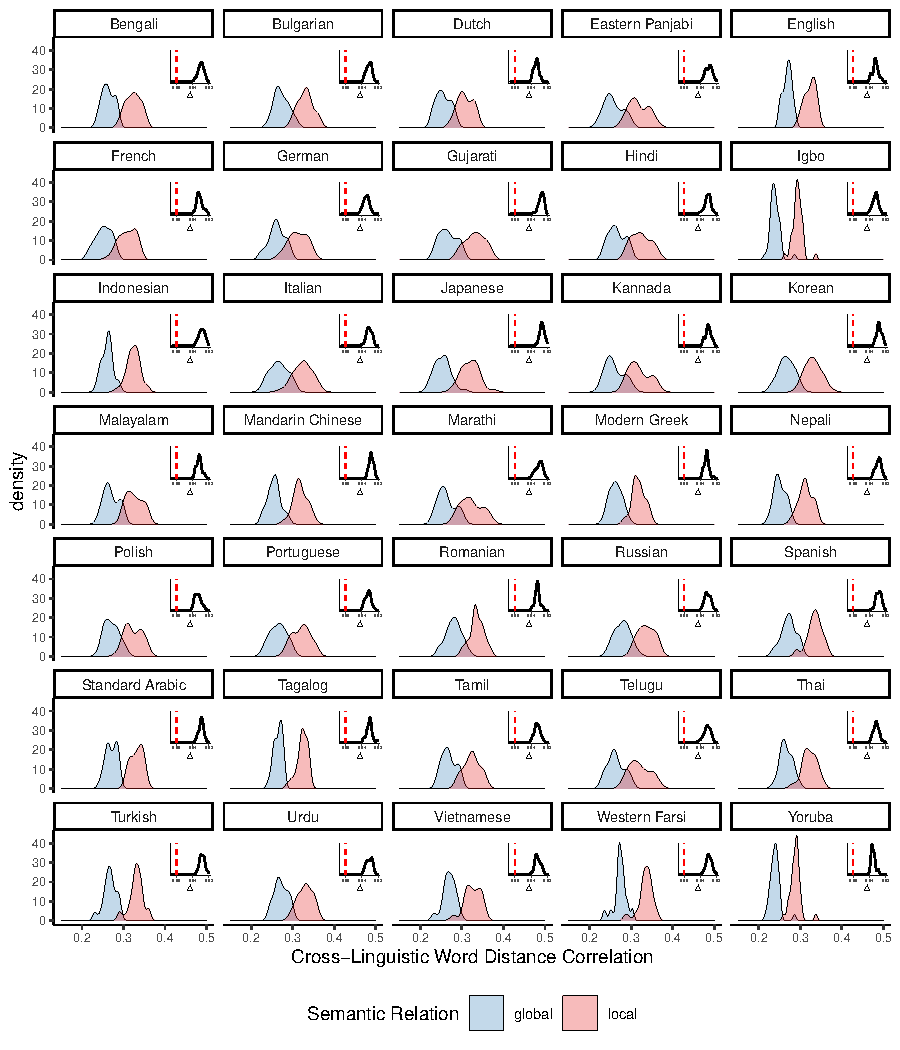
\includegraphics[width = 7in]{suppfigs/local_global_language_dist_ED_ETS.pdf}
         \caption{Distribution of local-global correlation difference by language, for TOEFL corpus. Each subplot shows the difference in correlation between local distances and global distances for one language with all other languages ($n$ = 34). The insets manifest the differences in the two distributions with the dashed red line signifying a difference of 0. These demonstrate that TOEFL local-global differences are not driven by outliers but appear largely balanced across all language combinations, with a consistent effect of roughly the same size across language comparisons.

}
\end{figure}


\pagebreak
 \clearpage
 
  %\section*{Fig. S20}

 \begin{figure}[h]
\centering
     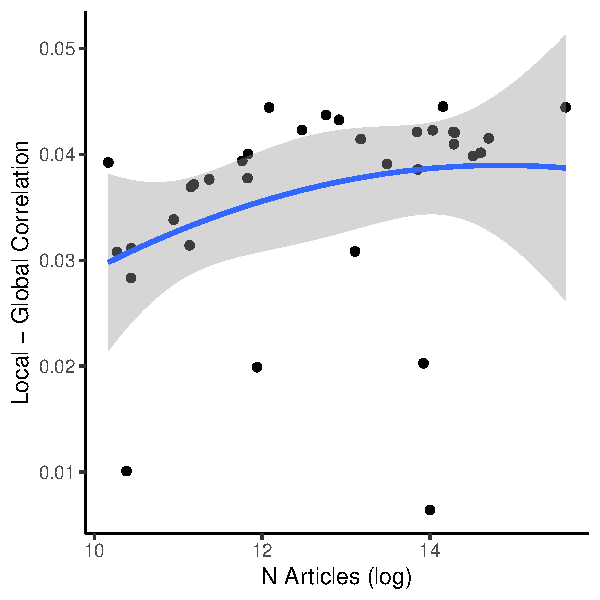
\includegraphics[width = 5in]{suppfigs/local_global_articles.pdf}
         \caption{Difference in cross-linguistic word distance correlations between local and global relations, as a function of the number of Wikipedia articles present for a given language \cite{wikispeakers}. Each point corresponds to a language.  Cross-linguistic word distance correlations are estimated from models trained on Wikipedia in each language. While in all languages local correlations are greater than global correlations, the difference is somewhat larger for languages for which more articles are available. This is almost certainly due to measurement error for local words. Smaller collections of articles will necessarily have smaller numbers of local (within-cluster) words, leading to higher variance and lower local-word correlations between languages. These lower localized correlations reduce the difference between local and global semantic distances. Nevertheless, when we split the languages in half by Wikipedia page number, we find that the significance of the relation holds for both small and large Wikipedia page languages.
}
\end{figure}

\pagebreak
 \clearpage
 
 %\section*{Fig. S21}
 
\begin{figure}[h]
\centering
     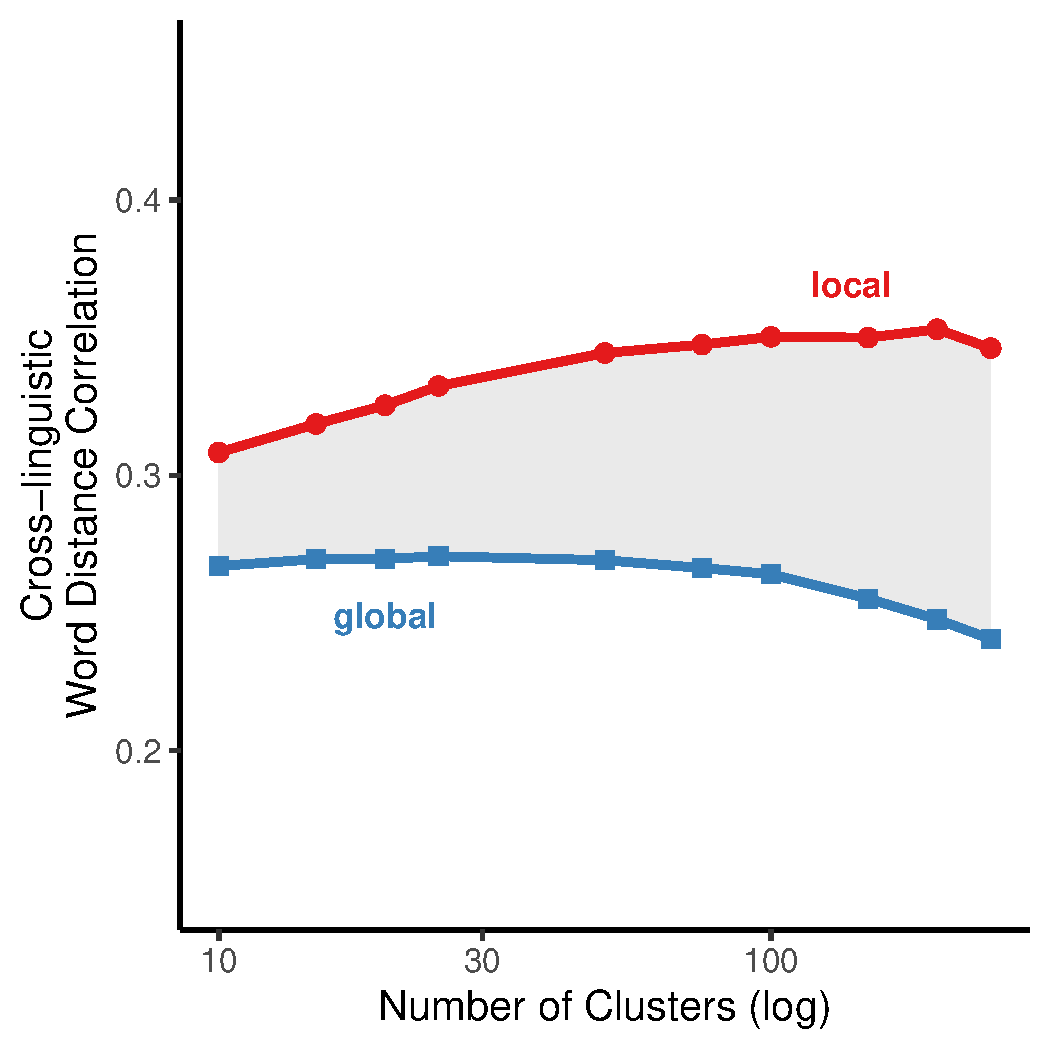
\includegraphics[width = 5in]{suppfigs/native_clustering_local_global}
         \caption{Cross-linguistic word distance correlations for local (red) versus global (blue) semantic comparison as a function of the number of semantic clusters using native model clusters for models trained on TOEFL essays. In Fig. 3D of the Main Text, we demonstrate that distances within clusters (local) are more correlated with each other cross-linguistically than word distances across clusters (global). This analysis was based on clusters defined by a model trained on English Wikipedia articles. Here, we replicate this pattern using clusters determined by models trained on native language text. For example, when comparing TOEFL essays from native Hindi and Mandarin speakers, we clustered words covering the Hindi and Chinese Wikipedia entries to capture how each language represents its knowledge base. Then we compared within Hindi-Wikipedia-clusters vs. between Hindi-Wikipedia-clusters for essays from native speakers of both languages; next we compared within Mandarin-Wikipedia-clusters vs. between Mandarin-Wikipedia clusters for the same essays; finally we averaged these differences. }
\end{figure}

















%\section*{Fig. S1}

\begin{table}[h]
\centering
\begin{tabular}{llp{1.5cm}p{1.8cm}p{1.3cm}p{1.3cm}p{1.3cm}p{1.3cm}}

  & &  Semantic   &  Grammatical   &  Physical   &  Climate  &  Lexical    &  Cultural  \\ 
  \hline
    \hline
{\it 35 languages} & Semantic  & 1.00 & & &  & \\ 
& Grammatical  & 0.55 & 1.00 &  & & \\ 
& Physical  & 0.52 & 0.46 & 1.00 &  & \\ 
& Climate  & 0.55 & 0.35 & 0.55 & 1.00 & \\ 
& Lexical  & 0.71 & 0.60 & 0.45 & 0.45 & 1.00 \\ 
   \hline
  % \hline
{\it 28 languages} &   Semantic  & 1.00 &  &  & &  & \\ 
 &Grammatical  & 0.61 & 1.00 &  &&  & \\ 
&Physical  & 0.52 & 0.53 & 1.00 & & &\\ 
& Climate  & 0.54 & 0.41 & 0.58 & 1.00  &  &\\ 
&  Lexical  & 0.73 & 0.63 & 0.47 & 0.49& 1.00 & \\
&    Cultural  & 0.69 & 0.47 & 0.49 & 0.59 & 0.72  & 1.00\\ 
      \hline
        \hline
\end{tabular}
   \caption{ {\it Top:} Pairwise correlations (Pearson's {\it r}) between language distances measures for all 35 languages (excluding cultural distance measure which has  missing data). {\it Bottom:} Pairwise correlations (Pearson's {\it r}) between language distance measures for the subset of 28 languages for which data is available for all 6 predictors. All correlations are significant at the $\alpha$ = .05 level using QAP tests.} 
\end{table}

\pagebreak
 \clearpage

 

 


\FloatBarrier



%\dataset{}{Data are available through the GitHub repository associated with the project: %\url{https://github.com/mllewis/SYSTEMSEM}}

% For your review copy (i.e., the file you initially send in for
% evaluation), you can use the {figure} environment and the
% \includegraphics command to stream your figures into the text, placing
% all figures at the end.  For the final, revised manuscript for
% acceptance and production, however, PostScript or other graphics
% should not be streamed into your compliled file.  Instead, set
% captions as simple paragraphs (with a \noindent tag), setting them
% off from the rest of the text with a \clearpage as shown  below, and
% submit figures as separate files according to the Art Department's
% instructions.

\pagebreak
 \clearpage
 
\bibliography{L2ETS_bib}

\end{document}
